
\documentclass[lettersize,journal]{IEEEtran}
\usepackage{amsmath,amssymb,amsfonts}
\usepackage{array}
\usepackage{booktabs}
\usepackage{multirow}

\usepackage{algorithm}
\usepackage{algorithmic}

\usepackage{graphicx}
\usepackage[cmyk]{xcolor}
\usepackage{textcomp}
\usepackage{soul}

% IEEE recommended sub-figures (use \subfloat, not subfigure environment)
% Use roman (same as main text) for sub-figure captions/labels
\usepackage[caption=false,font=normalsize,labelfont=rm,textfont=rm]{subfig}

\usepackage{url}
\usepackage{verbatim}
\usepackage{cite}
\usepackage{stfloats}

% CJK + hyperlinks/cleveref (order matters: hyperref -> cleveref)
\usepackage{xeCJK}
\usepackage{hyperref}
\usepackage{cleveref}


\hyphenation{op-tical net-works semi-conduc-tor IEEE-Xplore}
% updated with editorial comments 8/9/2021

\begin{document}

\title{KAMT: Knowledge-Augmented multi-modal learning based AD and relevant dementia(ADRD) diagnosis}



\author{IEEE Publication Technology,~\IEEEmembership{Staff,~IEEE,}
        
}

% The paper headers
\markboth{Trans}%
{Author \MakeLowercase{\textit{et al.}}: KAMTT}



\maketitle

\begin{abstract}
        For precision diagnosis, the model performance of deep learning approaches has an over-reliance on sample size and data quality.
        In this case, domain knowledge has played an essential role in enhancing the credibility and reliability of deep learning approaches, especially in precision medicine applications. Neuroimage samples and clinical metadata have been employed to conduct precision diagnostic models for ADRD and cognitive impairment. For the textual modality associated with AD and dementia, the semantic relations between biomedical entities could be applied as domain knowledge to guide the learning of deep neural networks. Under the MML framework, this work proposes the KAMT architecture to enhance prediction accuracy and credibility in ADRD diagnosis.   
        
\end{abstract}

\begin{IEEEkeywords}
	Clinical knowledge, multi-omics integration, ADRD diagnosis.
\end{IEEEkeywords}

\section{Introduction}
\label{sec:introduction}

    \textcolor{blue}{\IEEEPARstart{A}{ssessment} of brain diseases has become an important topic in precision medicine. For neurodegenerative diseases such as Parkinson's disease (PD) and Alzheimer's disease (AD), multimodal deep learning integrating diverse features has gradually become the mainstream approach in this field \cite{qiu2022multimodal,zhang2026multimodalpd}. Recent advanced frameworks have even attempted to ground diagnostic decisions in localized anatomy and clinical variables to improve transparency \cite{lin2025adlip,wood2026align}. Specifically, practical diagnostic pipelines typically involve extracting baseline information from Electronic Health Records (EHR)\cite{rajkomar2018scalable}, tracking the dynamic changes of clinical scales within Biomarkers (BM)\cite{marek2011parkinson}, and utilizing 3D-CNNs \cite{basaia2019automated} to preprocess Magnetic Resonance Imaging (MRI) for capturing localized microstructural patterns.}

    However, lacking prior guidance on underlying pathological mechanisms, purely data-driven models heavily rely on isolated numerical computations and image feature extraction. By ignoring the critical semantic associations between biomedical entities in medical records, these approaches suffer from severe overfitting and performance degradation\cite{lu2021knowledge} when applied to multi-center clinical cohorts with heterogeneous feature distributions.

    \textcolor{blue}{With efficient representations, the Knowledge-Augmented learning scheme could provide a way to improve the model performance as well as model explainability. It is noted that the quality of knowledge representations determines the prediction accuracy and model generalization ability in precision medicine \cite{chandak2023building}.}  \textcolor{blue}{Motivated by established works about large-scale Clinical knowledge graphs including SPOKE \cite{morris2023spoke} and PharmKG \cite{zheng2021pharmkg}, this work develops the dementia-specific knowledge graphs by extracting complicated causal relations between biomedical ontology that are associated with brain disease and cognitive decline.}

    \textcolor{blue}{Knowledge-augmented neural network learning architecture is another essential perspective in obtaining reliable predictions} from multimodal data. \textcolor{blue}{With external knowledge, Relational knowledge graphs were constructed to capture causal relations for biomedical entities that are associated with dementia and cognitive decline. For neurological disorders, essential ontologies such as vascular dynamics and immune regulation have been encoded in the triplets in large-scale biomedical KG \cite{zhao2026kgt,sim2024gtad}.}
    
\begin{itemize}
    \item High-quality knowledge representations have been extracted and exploited in disease prediction;
    \item Clinical knowledge-augmented learning scheme has been proposed to integrate augmented knowledge representations and multi-modal learning;
    \item  For dementia and cognitive impairment, clinic knowledge has been extracted as triplets and incorporated into multimodal learning network;
    \item External knowledge source was introduced to obtain high-quality domain knowledge in the diagnostic of ADRD, with the proposed X-KD strategy.
\end{itemize}




\section{Related Works}

\subsection{Multimodal Deep Learning for Dementia Diagnosis}

    Multimodal deep learning approaches have been widely used for assessing Alzheimer's disease and related dementia(ADRD) by jointly modeling clinical text and imaging phenotypes \cite{jin2026multimodal}. While attention-based fusion has improved representation capacity, purely data-driven models can still exhibit distribution shift and reduced generalization across sites/cohorts with heterogeneous acquisition protocols and feature distributions \cite{abugabah2025intelligent}. In addition, without explicit mechanistic priors, these models may rely on spurious within-modality correlations and underutilize clinically meaningful semantic links between medical entities and cognitive outcomes.

\subsection{Knowledge-Guided Multimodal Fusion Frameworks}

    Clinical knowledge graphs offer structured priors that can support multimodal learning. It is noted that directly incorporating large-scale, general-purpose KGs may introduce biological noise and dilute task-relevant signals. In contrast, domain-specific graphs built from local records can better match the target cohort yet often lack ontology breadth and transferability. These trade-offs motivate task-adaptive relational diagnostic KGs that balance specificity with external coverage.


    Multiple knowledge-enhanced multimodal models still follow a shallow fusion strategy, treating KG embeddings as independent vectors that are concatenated with image/text features near the output \cite{chen2023knowledge}, which can limit how knowledge shapes intermediate learning and cross-modal alignment. Recent diagnostic models therefore increasingly use Transformer-style self-/cross-attention to adaptively weight and align heterogeneous representations \cite{vaswani2017attention,kyritsis2025transformerfusionad,li2024hammf,du2025vitadreview,chen2026federatedvitad}. In this work, we address the gap between shallow knowledge injection and fine-grained fusion by introducing knowledge-augmented features into the cross/self-attention module, allowing KG information to act as an implicit constraint that guides multimodal representation learning.

    
\section{\textcolor{blue}{Clinically Guided Knowledge Augmentation with KAMT}}

    In precision diagnosis of brain diseases, knowledge graph embedding (KGE) methods aim to encode biomedical entities and their relations into a low-dimensional semantic space.
    Specifically, the KGE method learns low-rank entity representations by scoring observed triplets higher than corrupted ones. Representative models include TransE\cite{bordes2013translating}, DistMult, ComplEx\cite{trouillon2016complex}, and RotatE\cite{sun2019rotate}.

    \textcolor{blue}{We propose} a controlled relation graph refinement paradigm: task-specific multimodal seeds have been extracted and topological refinement has been conducted to build a dementia-oriented relational KG (DemRKG), \textcolor{blue}{which provides entity representations for downstream KAMT.}

\begin{comment}
The overall refinement and construction pipeline is illustrated in \cref{fig:dementia_hkg_flow}.

\begin{figure}[htbp]
    \centering
    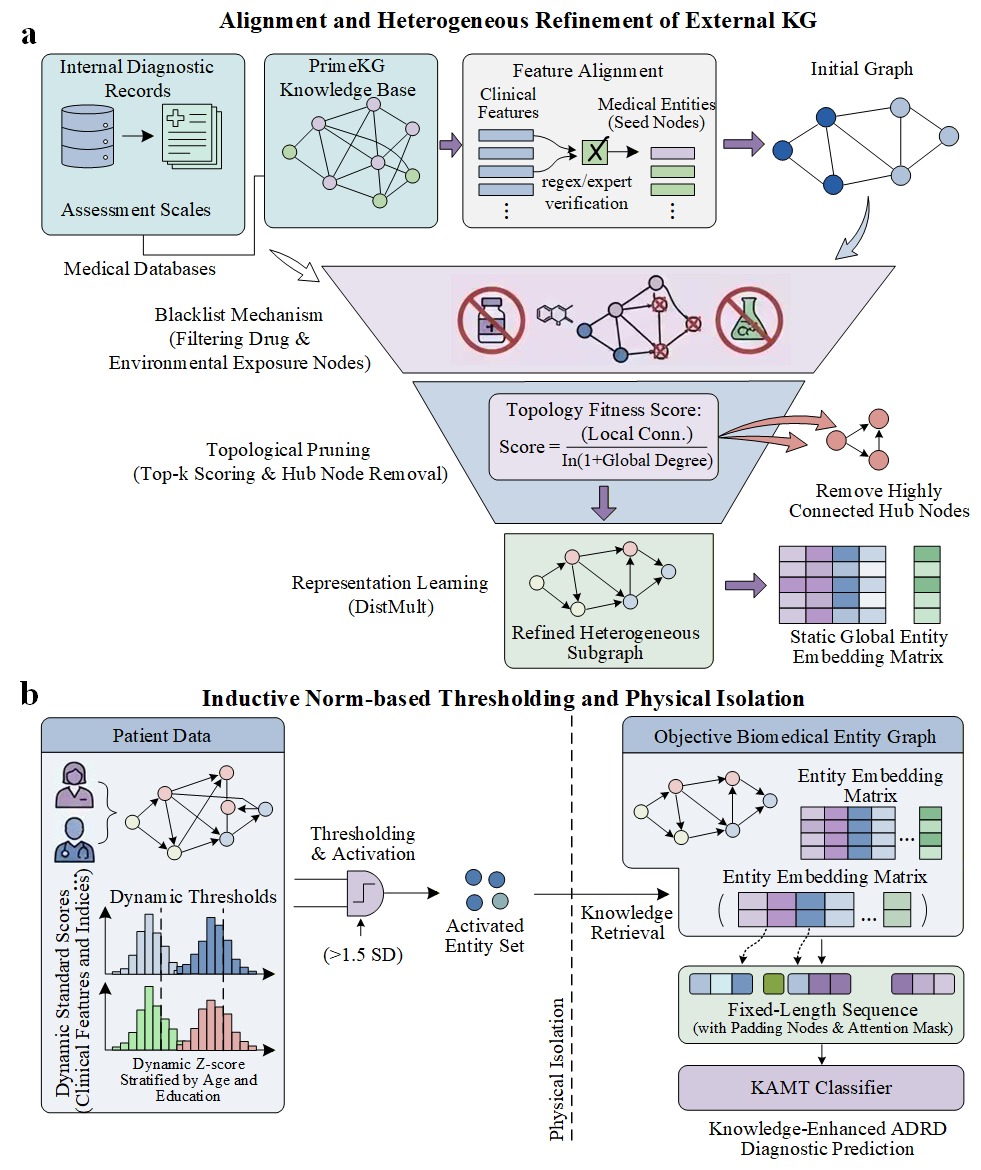
\includegraphics[width=\linewidth]{Figures/DementiaHKG流程图-EN.png}
    \caption{The construction, refinement, and patient-specific activation pipeline of DemRKG. (a) Alignment and heterogeneous refinement of the external KG, illustrating the topological pruning and DistMult representation learning. (b) Inductive norm-based thresholding and physical isolation for objective patient sequence generation.}
    \label{fig:dementia_hkg_flow}
\end{figure}
\end{comment}

\subsection{\textcolor{blue}{Refinement of DemRKG}}

\subsubsection{\textcolor{blue}{Clinical Seed Alignment}}

     \textcolor{blue}{Using dataset-specific clinical fields, we manually select medical keywords that reflect their diagnostic meaning. We search relevant entity types in PrimeKG $\mathcal{G}_0=(\mathcal{V}_0,\mathcal{R}_0,\mathcal{T}_0)$ for candidate entities and present the shortest names first for manual review. Selected standard entity names are entered into a dataset-specific field--entity dictionary and checked against PrimeKG. The validated pairs define $M:\mathcal{F}\rightarrow\mathcal{V}_0$, where $\mathcal{F}$ contains the matched clinical fields; their entities form $\mathcal{S}_{\mathrm{clinical}}$. In parallel, we manually select dataset-specific disease and molecular core candidates based on medical domain knowledge and retain those found in PrimeKG as $\mathcal{S}_{\mathrm{core}}$. The resulting dataset-level seed set is}
     \begin{equation}
     \mathcal{S}
     =
     \mathcal{S}_{\mathrm{clinical}}
     \cup
     \mathcal{S}_{\mathrm{core}}.
     \label{eq:seed_set}
     \end{equation}
     \textcolor{blue}{The seed set $\mathcal{S}$ serves as the starting point for subsequent graph refinement.}

\subsubsection{\textcolor{blue}{Degree-Aware Graph Pruning}}

    \textcolor{blue}{Starting from $\mathcal{S}$, we retrieve one-hop edges. Let $\mathcal{B}_{\mathrm{type}}$ and $\mathcal{B}_{\mathrm{rel}}$ denote the blacklisted entity types and relations. For an edge set $\mathcal{U}\subseteq\mathcal{T}_0$, we remove edges with a blacklisted endpoint type or relation:}
    \begin{equation}
        {\color{blue}
        \begin{aligned}
        \mathcal{U}_{\mathrm{clean}}=\mathcal{U}\setminus\{(h,r,t)\in\mathcal{U}:\;&
        \operatorname{type}(h)\in\mathcal{B}_{\mathrm{type}}\\
        &\lor\operatorname{type}(t)\in\mathcal{B}_{\mathrm{type}}\\
        &\lor r\in\mathcal{B}_{\mathrm{rel}}\}.
        \end{aligned}
        }
        \label{eq:blacklist_filter}
    \end{equation}
    \textcolor{blue}{We apply this filter to the one-hop edges, expand from the retained neighborhood to obtain candidate two-hop edges, and apply the same filter to these candidates. In particular, protein--protein interaction (PPI) edges connect proteins in the seed neighborhood to their interacting partners, providing molecular paths for capturing indirect associations with the clinical seeds} \cite{barabasi2011network,cheng2019network}. \textcolor{blue}{To reduce the influence of highly connected nodes in the expanded graph, we define the following specificity score:}

    \begin{equation}
        Score(w) = \frac{L(w)}{\ln(1 + G(w))}
        \label{eq:spec-score}
    \end{equation}
    where \textcolor{blue}{$L(w)$ counts distinct candidate source nodes connected to $w$}, and \textcolor{blue}{$G(w)$ counts records in which $w$ occurs at either endpoint in PrimeKG}. \textcolor{blue}{The numerator measures a candidate target's connectivity to multiple sources, while the denominator penalizes its global degree. For each source, we select the top-$k$ candidate edge records according to their target-node scores. We then merge the selected records with the filtered one-hop edges and remove duplicate records to obtain the refined triplets $\mathcal{T}$.}

\subsubsection{\textcolor{blue}{Relation-Trained Entity Representations}}

    \textcolor{blue}{Using the refined triplets $\mathcal{T}$ from DemRKG, we pre-train KG embeddings in $\mathbb{R}^d$ and generate negative samples by replacing tail entities. DistMult scores each triplet as $f(h,r,t)=\langle\mathbf e_h,\mathbf r_r,\mathbf e_t\rangle$. We optimize the embeddings using a margin-based ranking loss with $\gamma=1.0$:}

    \begin{equation}
        {\color{blue}
        \mathcal{L} = \frac{1}{|\mathcal{B}|}\sum_{(h,r,t)\in\mathcal{B}}
        \max\left(0,\gamma-f(h,r,t)+f(h,r,t')\right),
        }
        \label{eq:margin_loss}
    \end{equation}
    \textcolor{blue}{where $\mathcal{B}$ is a training batch and $t'$ is one randomly sampled replacement tail for each positive triple.}
    \textcolor{blue}{Training yields entity embeddings $\mathbf{E} \in \mathbb{R}^{|\mathcal{V}| \times d}$ and relation embeddings $\mathbf{R} \in \mathbb{R}^{|\mathcal{R}| \times d}$. The entity embeddings support subsequent patient-specific knowledge activation.}
    \textcolor{blue}{DemRKG's relation-trained entity embeddings supply the Keys for compatibility-energy computation and the Values for knowledge readout, while patient-specific activation determines the valid support $J_i$.}


\subsection{\textcolor{blue}{Multimodal encoding and patient-specific knowledge activation}}

    \subsubsection{\textcolor{blue}{Clinical feature grouping and encoding}}
    
    \textcolor{blue}{We divide the cleaned diagnostic tabular features} $\mathcal{D}_{\mathrm{clean}}$ \textcolor{blue}{into Electronic Health Records (EHR) and Biomarkers (BM) groups through} $f_{\mathrm{split}}$:

    
    \begin{equation}
        \mathcal{M}_{\mathrm{EHR}}, \mathcal{M}_{\mathrm{BM}} = f_{\mathrm{split}}(\mathcal{D}_{\mathrm{clean}})
        \label{eq:modality_split}
    \end{equation}


    \textcolor{blue}{EHR captures relatively stable demographic, medical-history, and genetic attributes, while BM comprises clinical scales reflecting changes in disease-related cognitive, behavioral, and motor functions.}
    
    \textcolor{blue}{Separate multi-layer perceptrons (MLPs) encode the EHR and BM features} \cite{wang2024unity}. \textcolor{blue}{A two-layer MLP computes the representation as follows:}
    
    \begin{equation}
    \mathbf{h} = \text{ReLU}(\text{BN}(\mathbf{W}_1 \mathbf{x} + \mathbf{b}_1))
    \label{eq:MLP_1}
    \end{equation}
    \begin{equation}
    \mathbf{z} = \text{ReLU}(\text{BN}(\mathbf{W}_2 \text{Dropout}(\mathbf{h}) + \mathbf{b}_2))
    \label{eq:MLP_2}
    \end{equation}

    where \textcolor{blue}{$\mathbf{W}_1$ and $\mathbf{W}_2$ are the weight matrices}, $\mathbf{b}_1$ and $\mathbf{b}_2$ are the corresponding bias terms, and BN denotes batch normalization. \textcolor{blue}{For subsequent knowledge queries, we denote the EHR and BM encoder outputs by $\mathbf h_{im}$ for patient $i$ and branch $m$.}

\subsubsection{\textcolor{blue}{Patient-specific knowledge activation}}

\textcolor{blue}{For patient $i$, we first apply the corresponding activation rule to each observed clinical field. The activated fields are then mapped to knowledge entities through $M$ and arranged into a fixed-length sequence:}
\begin{equation}
    {\color{blue}
    \begin{aligned}
    a_{if} &= \mathcal{A}_f(x_{if};\eta_f^{\mathrm{train}}),\\
    \nu_i &= \operatorname{Seq}_{L_{kg}}\bigl((M(f))_{f:a_{if}=1}\bigr),\\
    J_i &= \{j\in I_i:\nu_i(j)\in\mathcal{V}\},\\
    {\color{black}\mathbf{X}_{KG}^{(i)}[j]} &{\color{black}= \mathbf{E}_{\nu_i(j)}},\qquad j\in J_i.
    \end{aligned}
    }
    \label{eq:patient_activation}
\end{equation}

\textcolor{blue}{where $x_{if}$ is the observed value of field $f$, and $\mathcal{A}_f$ is its binary activation rule. The rule uses either training-set statistics $\eta_f^{\mathrm{train}}$ or predefined thresholds. We estimate the reference statistics from the training set, fix them, and apply them unchanged to the training, validation, and test sets. $\operatorname{Seq}_{L_{kg}}$ applies dataset-specific deduplication, truncation, and padding rules.}

\textcolor{blue}{$I_i=\{1,\ldots,L_{kg}\}$ indexes the sequence positions, and $\mathcal{V}$ is the entity set represented in $\mathbf{E}$. We fill positions outside $J_i$ with zero vectors and exclude them through the mask $\mathbf{m}_i$. Only positions in $J_i$ are used in the subsequent conditional free-energy computation for knowledge weighting.}

\textcolor{blue}{If $J_i=\varnothing$, we retain the zero-filled knowledge sequence and unmask its first position as a zero-input placeholder. The same adaptation and attention operations produce a response, which is integrated through the residual update.}


\subsubsection{\textcolor{blue}{MRI feature encoding}}
    
     \textcolor{blue}{Structural MRI provides complementary imaging information. After center cropping, the MRI volume is processed by a 3D-CNN consisting of convolutional, pooling, and fully connected layers} \cite{wen2020convolutional,tran2015c3d}. \textcolor{blue}{The MRI representation is obtained as}
     \begin{equation}
     {\color{blue}Z_{img} = \phi_{\mathrm{img}}\!\left(\operatorname{CenterCrop}(I)\right),}
     \label{eq:mri_projection}
     \end{equation}
     \textcolor{blue}{where $I$ denotes the input MRI volume and $\phi_{\mathrm{img}}$ denotes the image encoder. The MRI branch maps $Z_{img}$ to $\mathbf h_{i,\mathrm{MRI}}$ for subsequent knowledge queries.}

\subsection{\textcolor{blue}{Knowledge weighting, injection, and multimodal prediction}}

    \textcolor{blue}{KAMT uses the patient-specific knowledge sequence to augment the EHR, BM, and MRI representations before multimodal fusion}, as summarized in \cref{fig:KAMT_framework}.

    \begin{figure*}[!t]
        \centering
        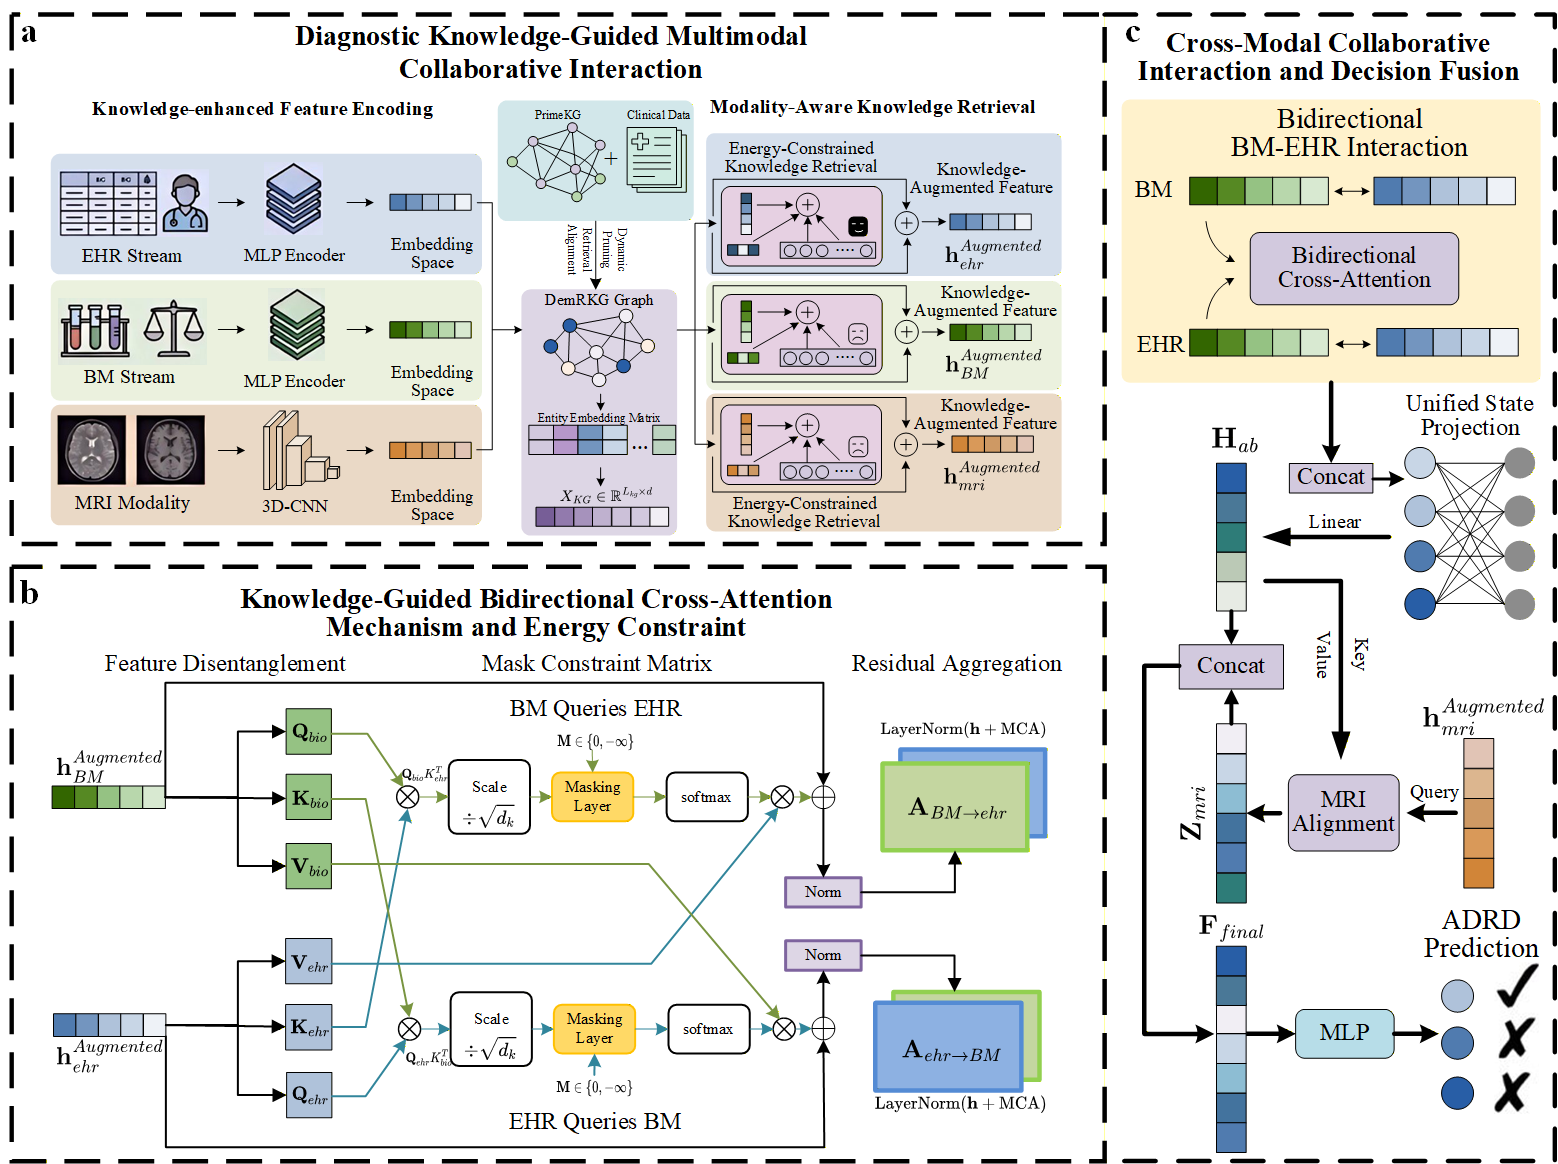
\includegraphics[width=\textwidth]{Figures/KAMT-Trans框架图.png}
        \caption{Overall architecture of KAMT. (a) Knowledge-Augmented encoding and modality-aware retrieval from KG sub-graphs. (b) Masked cross-attention for knowledge injection and the proposed energy-constrained refinement. (c) BM-EHR collaboration guides MRI alignment; the final prediction is made from the fused low-level state and aligned MRI representation.}
        \label{fig:KAMT_framework}
    \end{figure*}

    %\textcolor{purple}{Roles and functions of energy-constrained refinement pathway are still unclear.}
    \textcolor{blue}{The three branches query the same patient knowledge sequence through branch-specific adapters and attention mappings. The conditional free energy below determines the knowledge weights for each branch.}

\subsubsection{\textcolor{blue}{Conditional free energy and knowledge weighting}}

    \textcolor{blue}{For patient $i$ and branch $m\in\{\mathrm{EHR},\mathrm{BM},\mathrm{MRI}\}$, a learned projection maps the encoded representation $\mathbf h_{im}$ to the Query. The branch-specific adapter $A_m$ transforms the DemRKG embeddings, and learned projections map its output to Keys and Values. For a single attention head:}
    \begin{equation}
        {\color{blue}
        \begin{aligned}
        g_{imj}&=A_m(\mathbf X_{KG}^{(i)}[j]),\\
        q_{im}&=W_m^Q\mathbf h_{im}+b_m^Q,\\
        k_{imj}&=W_m^Kg_{imj}+b_m^K,\\
        v_{imj}&=W_m^Vg_{imj}+b_m^V.
        \end{aligned}
        }
        \label{eq:knowledge_qkv}
    \end{equation}

    \textcolor{blue}{On the nonempty patient support $J_i$, the feasible weights lie in $\Delta(J_i)=\{\alpha\in\mathbb R_+^{L_{kg}}:\sum_j\alpha_j=1,\ \alpha_j=0\ (j\notin J_i)\}$. Using the uniform reference $u_i(j)=1/|J_i|$ and compatibility energy $\epsilon_{imj}=-q_{im}^{\mathsf T}k_{imj}/\sqrt{d_k}$, where $d_k$ is the Key dimension per head, the knowledge weights minimize the conditional free energy:}
    \begin{equation}
        {\color{blue}
        \boxed{
        \begin{aligned}
        \alpha_{im}^{*}&=\arg\min_{\alpha\in\Delta(J_i)}\mathcal F_{im}(\alpha),\\
        \mathcal F_{im}(\alpha)&=-\sum_{j\in J_i}\alpha_j
        \frac{q_{im}^{\mathsf T}k_{imj}}{\sqrt{d_k}}\\
        &\quad+D_{\mathrm{KL}}(\alpha\Vert u_i).
        \end{aligned}
        }
        }
        \label{eq:energy_min}
    \end{equation}

    \textcolor{blue}{The energy term favors entities compatible with the current modality representation, while the KL term regularizes the concentration of knowledge weights over the activated support. DemRKG's relation-trained embeddings enter the energy through the Keys, while patient activation restricts allocation to $J_i$.}

    \textcolor{blue}{For fixed Queries and Keys, the unique minimizer is}
    \begin{equation}
        {\color{blue}
        \begin{aligned}
        \alpha_{imj}^{*}&=
        \begin{cases}
        \displaystyle\frac{e^{-\epsilon_{imj}}}
        {\sum_{\ell\in J_i}e^{-\epsilon_{im\ell}}},&j\in J_i,\\[6pt]
        0,&j\notin J_i,
        \end{cases}\\
        \mathcal F_{im}(\alpha)-\mathcal F_{im}(\alpha^*)
        &=D_{\mathrm{KL}}(\alpha\Vert\alpha^*)\geq0.
        \end{aligned}
        }
        \label{eq:knowledge_optimum}
    \end{equation}
    \textcolor{blue}{Substituting the energy definition gives masked softmax:}
    \begin{equation}
        {\color{blue}
        \alpha_{im}^*=\operatorname{softmax}
        \left(\frac{K_{im}^{\mathsf T}q_{im}}{\sqrt{d_k}}+M_i\right),
        }
        \label{eq:knowledge_weights}
    \end{equation}
    \textcolor{blue}{where $K_{im}=[k_{im1},\ldots,k_{imL_{kg}}]$, and $M_i(j)=0$ for $j\in J_i$ or $-\infty$ otherwise. The weights $\alpha_{im}^*$ then control Value readout.}

\subsubsection{\textcolor{blue}{Knowledge readout and residual update}}

    \textcolor{blue}{For patient $i$ with nonempty support $J_i$, each of the $H$ attention heads uses the optimal weights $\alpha_{im}^{(a)*}$ from \cref{eq:knowledge_weights} to aggregate the corresponding Values. The head outputs are concatenated and projected to obtain the knowledge response:}
    
    \begin{equation}
        {\color{blue}
        \begin{aligned}
        \mathbf{z}_{im}^{kg}&=W_m^O\operatorname{Concat}_{a=1}^{H}\left(
        \sum_{j\in J_i}\operatorname{DropAttn}
        (\alpha_{im}^{(a)*})_j v_{imj}^{(a)}\right)\\
        &\quad+b_m^O,
        \end{aligned}
        }
        \label{eq:knowledge_response}
    \end{equation}

    \textcolor{blue}{where $\operatorname{DropAttn}$ applies attention-weight dropout during training and is the identity at inference; $W_m^O,b_m^O$ are the output projection parameters. The optimality in \cref{eq:knowledge_optimum} applies to the weights before this dropout.}
    \textcolor{blue}{When $J_i=\varnothing$, each head instead reads the first zero-input placeholder, whose attention weight is 1 before dropout. The resulting response is integrated through the same residual update.}

    Clinical knowledge \textcolor{blue}{is integrated by residual addition and layer normalization}:
    \begin{equation}
    \mathbf{h}_{\textcolor{blue}{i}m}^{Augmented} = \mathrm{LayerNorm}(\mathbf{h}_{\textcolor{blue}{i}m} + \mathbf{z}_{\textcolor{blue}{i}m}^{kg})
    \end{equation}

\subsubsection{\textcolor{blue}{Multimodal fusion and classification}}

    Using the augmented \textcolor{blue}{BM} and EHR features, KAMT performs bidirectional cross-attention\textcolor{blue}{, with Queries, Keys, and Values obtained from learned mappings of the augmented features}:
    
    \begin{equation}
        \begin{aligned}
        \mathbf{A}_{BM \rightarrow ehr} &= \mathrm{LayerNorm}(\mathbf{h}_{BM}^{Augmented} + \mathrm{MCA}(\mathbf{Q}_{BM}, \mathbf{K}_{ehr}, \mathbf{V}_{ehr})), \\
        \mathbf{A}_{ehr \rightarrow BM} &= \mathrm{LayerNorm}(\mathbf{h}_{ehr}^{Augmented} + \mathrm{MCA}(\mathbf{Q}_{ehr}, \mathbf{K}_{BM}, \mathbf{V}_{BM})).
        \end{aligned}
        \label{eq:bidirectional_mca}
    \end{equation}

    \textcolor{blue}{The bidirectional outputs are concatenated and mapped by $P_{ab}$, which comprises Linear, ReLU, and Dropout layers, to obtain the joint clinical representation:}
    
    \begin{equation}
        \mathbf{H}_{ab} = \textcolor{blue}{P_{ab}}\Big(\big[\mathrm{Squeeze}(\mathbf{A}_{BM \rightarrow ehr}) \parallel \mathrm{Squeeze}(\mathbf{A}_{ehr \rightarrow BM})\big]\Big).
        \label{eq:hab_def}
    \end{equation}


    The augmented MRI features \textcolor{blue}{are mapped to the Query for cross-attention with} $\mathbf{H}_{ab}$ \textcolor{blue}{as the Key and Value inputs:}
    
    \begin{equation}
        \mathbf{Z}_{mri} = \mathrm{LayerNorm}(\mathbf{h}_{mri}^{Augmented} + \mathrm{MCA}(\mathbf{Q}_{mri}, \mathbf{H}_{ab}, \mathbf{H}_{ab})).
        \label{eq:mri_alignment}
    \end{equation}

    \textcolor{blue}{We concatenate} $\mathbf{H}_{ab}$ and $\mathbf{Z}_{mri}$ \textcolor{blue}{to form the joint latent representation:}

    \begin{equation}
    \mathbf{F}_{final} = [ \mathrm{Squeeze}(\mathbf{H}_{ab}) \parallel \mathrm{Squeeze}(\mathbf{Z}_{mri}) ].
    \label{eq:final_fusion}
    \end{equation}

    \textcolor{blue}{An MLP classifier maps the fused representation $\mathbf{F}_{final}$ to logits $z_{i,c}$, which Softmax converts to class probabilities:}
    
    \begin{equation}
        \hat{y}_{i,c} = \frac{\exp(z_{i,c})}{\sum_{j=1}^{C} \exp(z_{i,j})}
        \label{eq:softmax}
    \end{equation}

    We optimize a $C$-class cross-entropy loss over a batch of size $B$:
    
    \begin{equation}
        \mathcal{L}_{CE} = - \frac{1}{B} \sum_{i=1}^{B} \sum_{c=1}^{C} y_{i,c} \log(\hat{y}_{i,c})
        \label{eq:cross_entropy}
    \end{equation}

    where $y_{i,c}$ is the one-hot ground-truth label. \textcolor{blue}{We apply} $L_2$ regularization to learnable parameters $\theta$, yielding the objective:
    
    \begin{equation}
        \mathcal{L}_{KAMT} = \mathcal{L}_{CE} + \lambda \sum_{w \in \theta} w^2
        \label{eq:total_loss}
    \end{equation}

    \textcolor{blue}{where $\lambda$ is the regularization coefficient. We optimize \cref{eq:total_loss} using Adam \cite{kingma2014adam}. The conditional free energy in \cref{eq:energy_min} determines $\alpha^*$ during each forward pass; these weights affect classification through Value readout, residual updates, and multimodal fusion.}

\section{Experimental outcomes and analysis}

\subsection{Dataset Descriptions}

% TODO(method-audit): 核对并统一常模估计与分类训练的患者划分：NACC 图构建 notebook 使用 seed 42 的 70/10/20 划分，分类 notebook 使用 seeds 32、30 的两次 8:2 划分（约 64/16/20）。
% 与第三章 eq:patient_activation 的训练集统计量定义对应；实验配置应采用生成论文结果的实际划分，并让常模估计和分类训练共用该划分。
    This study used four different datasets: ADNI\cite{weiner2013adni}, NACC\cite{beekly2007nacc}, AIBL\cite{ellis2009aibl}, and PPMI\cite{marek2011ppmi}. All datasets are first divided into an initial training set and a clean test set in an 8:2 ratio. Then, the initial training set is divided into a final training set and a validation set in an 8:2 ratio. The sample distribution and scale statistics of the datasets are summarized in \cref{tab:dataset_statistics}.

    \begin{table}[htbp]
        \centering
        \caption{Descriptions of the benchmark datasets in ADRD diagnosis.}
        \label{tab:dataset_statistics}
        \begin{tabular}{llccc}
            \toprule
            \textbf{Dataset} & \textbf{Task} & \textbf{Class} & \textbf{Count} & \textbf{Total} \\
            \midrule
            \multirow{3}{*}{ADNI} & \multirow{3}{*}{3-Class} & NC & 211 & \multirow{3}{*}{837} \\
            & & MCI & 475 & \\
            & & AD & 151 & \\
            \midrule
            \multirow{3}{*}{NACC} & \multirow{3}{*}{3-Class} & NC & 2,116 & \multirow{3}{*}{3,708} \\
            & & MCI & 879 & \\
            & & AD & 713 & \\
            \midrule
            \multirow{3}{*}{AIBL} & \multirow{3}{*}{3-Class} & NC & 358 & \multirow{3}{*}{516} \\
            & & MCI & 86 & \\
            & & AD & 72 & \\
            \midrule
            \multirow{4}{*}{PPMI} & \multirow{4}{*}{4-Class} & Control & 125 & \multirow{4}{*}{409} \\
            & & PD & 132 & \\
            & & SWEDD & 72 & \\
            & & Prodromal & 80 & \\
            \bottomrule
        \end{tabular}
    \end{table}

\subsection{Knowledge Extraction and Graph Visualization}

% \subsubsection{Knowledge Representation Extraction}

    Taking NACC as an example, the corresponding DemRKG was built by aligning 61 clinical/demographic features to PrimeKG entities. Clinical tests (e.g., Boston Naming Test; Trail Making Test A) are mapped to phenotype nodes (e.g., aphasia, executive dysfunction), while irrelevant domains (e.g., drug exposure/off-label use) are filtered via a global blacklist. We then collect the one-hop neighborhoods of these seeds and retain 17,666 cleaned edges. A two-hop expansion further selects topologically relevant nodes (top-5 truncation), adding 28,742 expansion edges. The resulting DemRKG contains 6,547 entities over 17 relation types, with 42,909 triples.

    Patient data are integrated via demographic standardization. We split NACC into train/test/validation with a 7:2:1 ratio. Within the training NC cohort, baseline norms are stratified by age and education. A feature node is activated when the corresponding score deviates from its norm by $>1.5\sigma$; for 2-hop nodes connected to 1-hop nodes, only the 5 nodes with the highest importance scores are selected. Each patient sequence is capped at length 45. This workflow maps 3,383/3,708 individuals and yields 30,335 valid feature maps for downstream modeling.

%\subsubsection{Graph Scale Statistics}
    
    \cref{tab:kg_statistics} summarizes the KG scales. PrimeKG is orders of magnitude larger ($>50$k entities; millions of triples) and can introduce semantic overload, adding peripheral noise to KAMT's cross-attention. In contrast, CustomKG grows with dataset feature coverage and cohort size, while DemRKG augments CustomKG with disease-relevant micro-level entities (e.g., genes/proteins) to balance coverage and specificity.
    \begin{table}[!t]
    \centering
    \caption{Knowledge Graph Scale Statistics}
    \label{tab:kg_statistics}
    \setlength{\tabcolsep}{8pt}
    \renewcommand{\arraystretch}{1.15}
    \begin{tabular}{c c r r}
    \hline
    \textbf{Dataset} & \textbf{Graph Type} & \textbf{Entities} & \textbf{Triplets (Edges)} \\
    \hline
    \multirow{3}{*}{ADNI} & CustomKG & 1,103  & 38,106 \\
                        & DemRKG   & 4,099  & 23,630 \\
                        & PrimeKG  & 52,532 & 3,743,954 \\
    \hline
    \multirow{3}{*}{AIBL} & CustomKG & 560    & 3,612 \\
                        & DemRKG   & 3,894  & 22,621 \\
                        & PrimeKG  & 50,061 & 3,712,962 \\
    \hline
    \multirow{3}{*}{NACC} & CustomKG & 4,003  & 291,673 \\
                        & DemRKG   & 6,547  & 42,909 \\
                        & PrimeKG  & 65,728 & 6,033,272 \\
    \hline
    \multirow{3}{*}{PPMI} & CustomKG & 677    & 16,410 \\
                        & DemRKG   & 2,497  & 13,050 \\
                        & PrimeKG  & 53,195 & 4,230,076 \\
    \hline
    \end{tabular}
    \end{table}

% \subsubsection{DemRKG Visualization}
    
    \cref{fig:dementia_viz} shows that DemRKG forms multiple dense local clusters and includes heterogeneous biomedical entities (genes, proteins, cellular components, molecular functions). Compared with phenotype-only planar graphs, this heterogeneous structure reflects the integration of external medical knowledge with patient-specific features, and provides links from macroscopic symptoms to microscopic mechanisms.

    \begin{figure}[!t]
        \centering
        \subfloat[NACC]{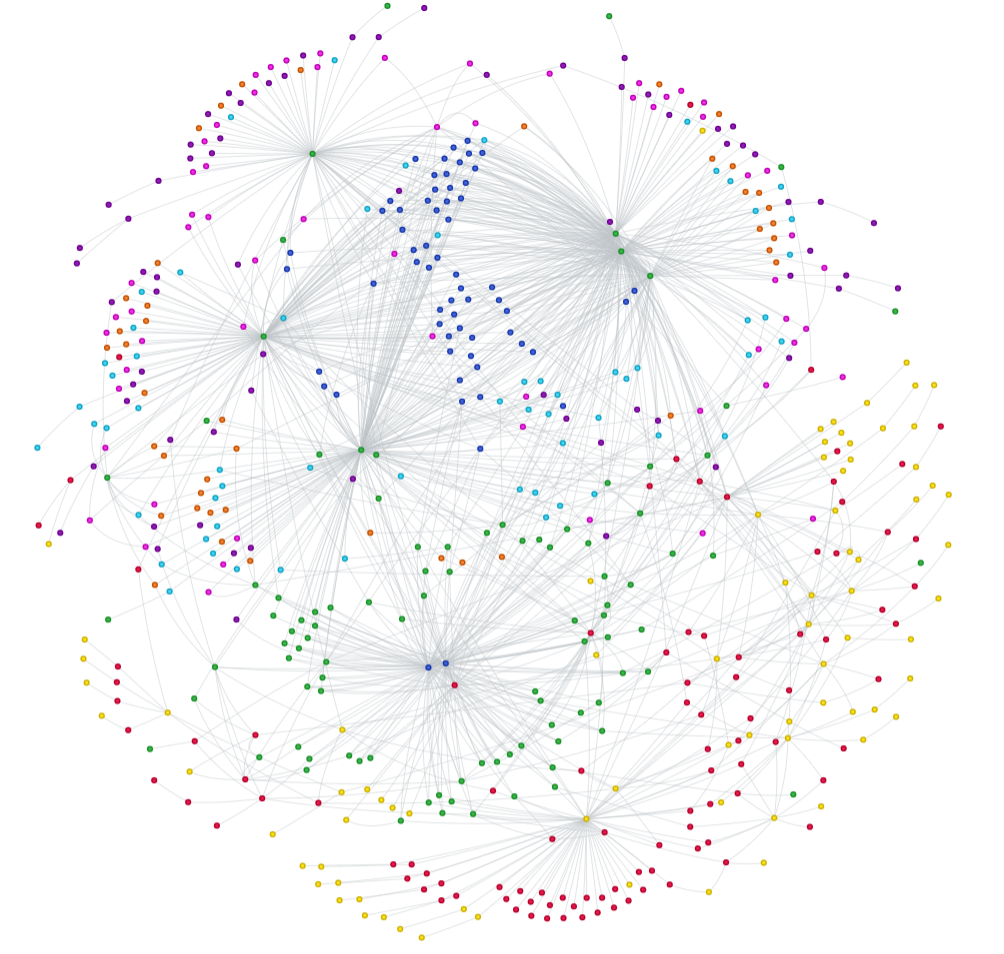
\includegraphics[width=0.48\linewidth]{Figures/NACC-DementiaHKG.png}}\hfill
        \subfloat[ADNI]{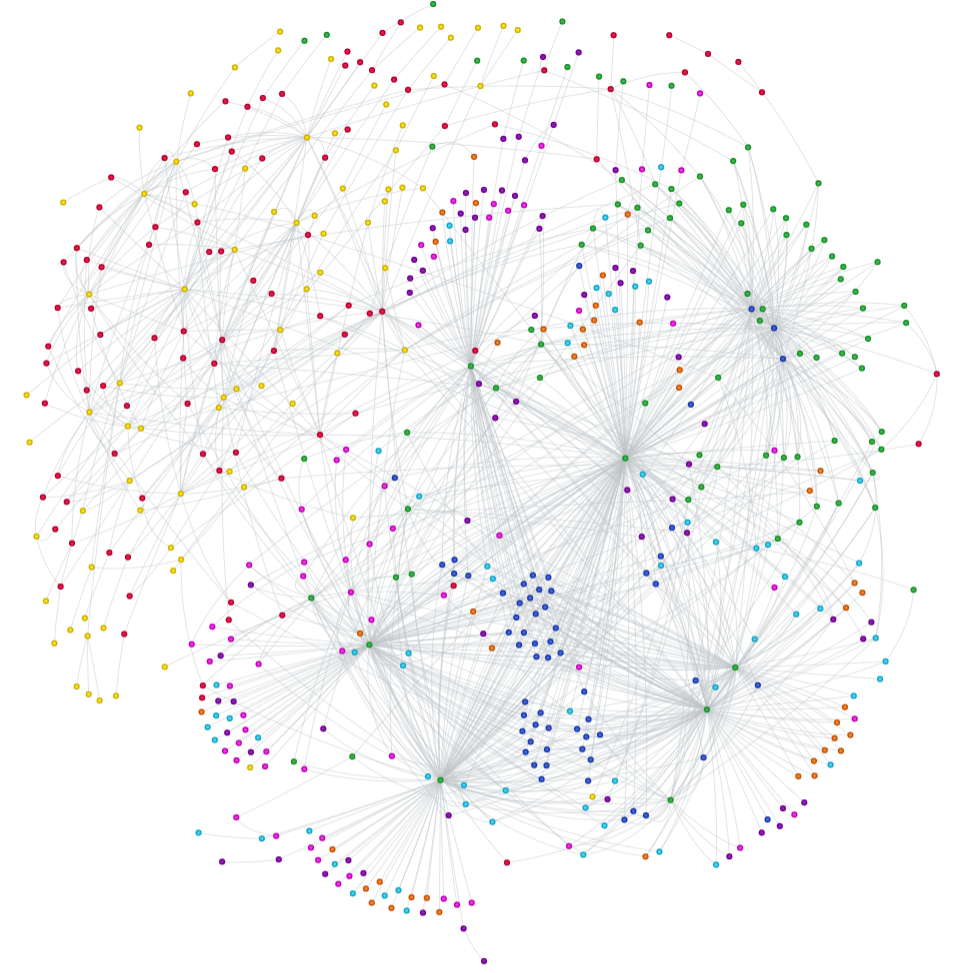
\includegraphics[width=0.48\linewidth]{Figures/ADNI-DementiaHKG.png}}\\
        \subfloat[PPMI]{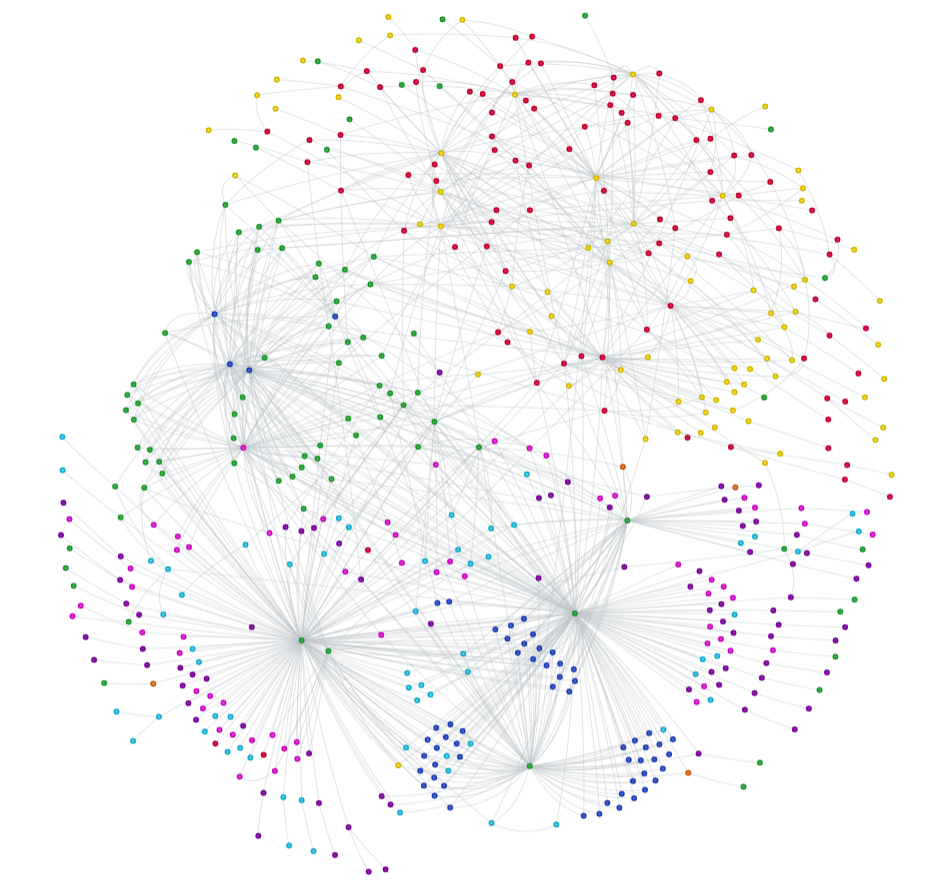
\includegraphics[width=0.48\linewidth]{Figures/PPMI-DementiaHKG.png}}\hfill
        \subfloat[AIBL]{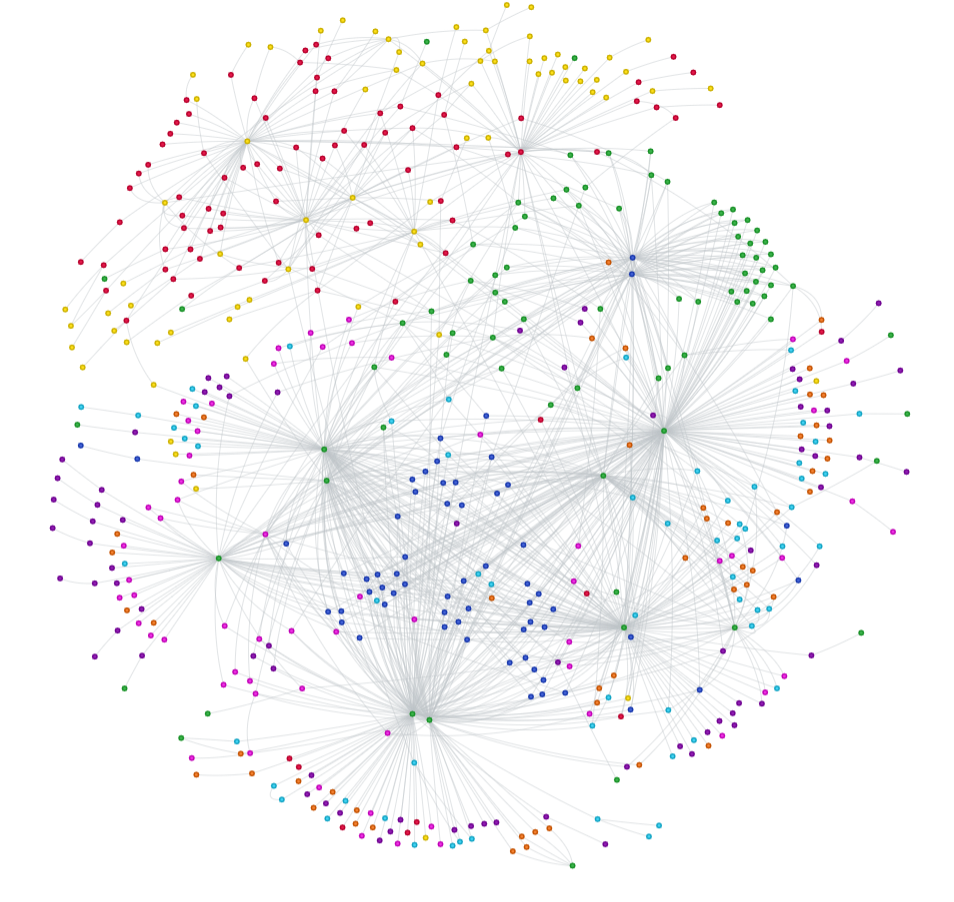
\includegraphics[width=0.48\linewidth]{Figures/AIBL-DementiaHKG.png}}
        \caption{Visualization of DemRKG across datasets: integrating multi-dimensional microscopic entities such as genes, proteins, and diseases.}
        \label{fig:dementia_viz}
    \end{figure}




\subsection{Performance Comparison}

   \begin{table*}[htbp]
\centering
\caption{Performance comparison of different methods on the AIBL, ADNI, NACC, and PPMI benchmarks}
\label{tab:performance_comparison}
\renewcommand{\arraystretch}{1.2} 
\begin{tabular}{llcccccc}
\toprule
\multirow{2}{*}{\textbf{Dataset}} & \multirow{2}{*}{\textbf{Metric}} & \textbf{MM-Trans} & \textbf{MM-Trans} & \textbf{AlignMamba} & \textbf{CAMera} & \textbf{KGT} & \textbf{KAMT} \\
 &  & \textbf{(Bi-modal)} & \textbf{(Tri-modal)} & \textbf{(Tri-modal)} & \textbf{(Tri-modal)} & \textbf{(TransE)} & \textbf{(DemRKG)} \\
\midrule
\multirow{5}{*}{\rotatebox{90}{AIBL}} 
& Accuracy  & 0.5402 $\pm$ 0.0423 & 0.4816 $\pm$ 0.0311 & 0.6204 $\pm$ 0.1238 & 0.6449 $\pm$ 0.1076 & 0.6843 $\pm$ 0.0387 & \textbf{0.8289 $\pm$ 0.0101} \\
& Precision & 0.3704 $\pm$ 0.0542 & 0.4806 $\pm$ 0.0416 & 0.6770 $\pm$ 0.1151 & 0.6692 $\pm$ 0.0732 & 0.5283 $\pm$ 0.1378 & \textbf{0.6977 $\pm$ 0.0253} \\
& Recall    & 0.3725 $\pm$ 0.0458 & 0.4474 $\pm$ 0.0384 & 0.6120 $\pm$ 0.1302 & 0.6462 $\pm$ 0.1114 & 0.4524 $\pm$ 0.0416 & \textbf{0.6912 $\pm$ 0.0253} \\
& F1 Score  & 0.3592 $\pm$ 0.0489 & 0.4146 $\pm$ 0.0603 & 0.5940 $\pm$ 0.1399 & 0.6175 $\pm$ 0.1046 & 0.4419 $\pm$ 0.0305 & \textbf{0.6772 $\pm$ 0.0229} \\
& AUC-ROC   & 0.6173 $\pm$ 0.0312 & 0.4916 $\pm$ 0.0245 & 0.6889 $\pm$ 0.1049 & 0.7292 $\pm$ 0.0514 & 0.7046 $\pm$ 0.0366 & \textbf{0.8660 $\pm$ 0.0259} \\
\midrule
\multirow{5}{*}{\rotatebox{90}{ADNI}} 
& Accuracy  & 0.5210 $\pm$ 0.0991 & 0.5770 $\pm$ 0.0526 & 0.5996 $\pm$ 0.0352 & 0.5676 $\pm$ 0.0263 & 0.6298 $\pm$ 0.0632 & \textbf{0.8299 $\pm$ 0.0112} \\
& Precision & 0.4242 $\pm$ 0.1345 & 0.5709 $\pm$ 0.0760 & 0.5732 $\pm$ 0.0758 & 0.4912 $\pm$ 0.1211 & 0.6011 $\pm$ 0.0848 & \textbf{0.8183 $\pm$ 0.0045} \\
& Recall    & 0.4139 $\pm$ 0.0543 & 0.5351 $\pm$ 0.0441 & 0.4697 $\pm$ 0.0926 & 0.4108 $\pm$ 0.0791 & 0.5633 $\pm$ 0.0734 & \textbf{0.8023 $\pm$ 0.0232} \\
& F1 Score  & 0.3779 $\pm$ 0.0880 & 0.5232 $\pm$ 0.0392 & 0.4350 $\pm$ 0.1224 & 0.3543 $\pm$ 0.1027 & 0.5650 $\pm$ 0.0815 & \textbf{0.8085 $\pm$ 0.0143} \\
& AUC-ROC   & 0.5626 $\pm$ 0.0506 & 0.7493 $\pm$ 0.0163 & 0.7535 $\pm$ 0.0262 & 0.6692 $\pm$ 0.0318 & 0.7696 $\pm$ 0.0620 & \textbf{0.9456 $\pm$ 0.0069} \\
\midrule
\multirow{5}{*}{\rotatebox{90}{NACC}} 
& Accuracy  & 0.5638 $\pm$ 0.0061 & 0.6540 $\pm$ 0.0041 & 0.6193 $\pm$ 0.0060 & 0.5897 $\pm$ 0.0183 & 0.7360 $\pm$ 0.0022 & \textbf{0.8067 $\pm$ 0.0102} \\
& Precision & 0.2474 $\pm$ 0.0558 & 0.5470 $\pm$ 0.0129 & 0.5751 $\pm$ 0.0105 & 0.5565 $\pm$ 0.0516 & 0.6574 $\pm$ 0.0148 & \textbf{0.7674 $\pm$ 0.0126} \\
& Recall    & 0.3364 $\pm$ 0.0046 & 0.5285 $\pm$ 0.0084 & 0.4561 $\pm$ 0.0259 & 0.3679 $\pm$ 0.0320 & 0.6387 $\pm$ 0.0068 & \textbf{0.7395 $\pm$ 0.0180} \\
& F1 Score  & 0.2591 $\pm$ 0.0153 & 0.4962 $\pm$ 0.0080 & 0.4540 $\pm$ 0.0459 & 0.3060 $\pm$ 0.0498 & 0.6302 $\pm$ 0.0221 & \textbf{0.7486 $\pm$ 0.0150} \\
& AUC-ROC   & 0.5695 $\pm$ 0.0111 & 0.7020 $\pm$ 0.0034 & 0.5981 $\pm$ 0.0366 & 0.5034 $\pm$ 0.0375 & 0.8242 $\pm$ 0.0031 & \textbf{0.9274 $\pm$ 0.0042} \\
\midrule
\multirow{5}{*}{\rotatebox{90}{PPMI}} 
& Accuracy  & 0.3227 $\pm$ 0.0564 & 0.4212 $\pm$ 0.0581 & 0.4927 $\pm$ 0.0462 & 0.3788 $\pm$ 0.1291 & 0.3446 $\pm$ 0.0637 & \textbf{0.6185 $\pm$ 0.0125} \\
& Precision & 0.1501 $\pm$ 0.0485 & 0.2653 $\pm$ 0.0494 & 0.4027 $\pm$ 0.1536 & 0.2818 $\pm$ 0.1715 & 0.3575 $\pm$ 0.0869 & \textbf{0.6084 $\pm$ 0.0621} \\
& Recall    & 0.2551 $\pm$ 0.0418 & 0.3647 $\pm$ 0.0631 & 0.4612 $\pm$ 0.0565 & 0.3390 $\pm$ 0.1108 & 0.3264 $\pm$ 0.0493 & \textbf{0.5462 $\pm$ 0.0084} \\
& F1 Score  & 0.1812 $\pm$ 0.0457 & 0.2651 $\pm$ 0.0709 & 0.4101 $\pm$ 0.1117 & 0.2291 $\pm$ 0.1258 & 0.3007 $\pm$ 0.0553 & \textbf{0.5166 $\pm$ 0.0182} \\
& AUC-ROC   & 0.5345 $\pm$ 0.0222 & 0.6740 $\pm$ 0.0827 & 0.6444 $\pm$ 0.1027 & 0.6580 $\pm$ 0.1548 & 0.5842 $\pm$ 0.0631 & \textbf{0.8308 $\pm$ 0.0075} \\
\bottomrule
\end{tabular}
\end{table*}

    As shown in \cref{tab:performance_comparison}, the impact of injecting KG signals is dataset-dependent for vanilla KG encoders, but becomes consistently beneficial under our knowledge-guided design. Specifically, the translation-based baseline KGT (TransE)~\cite{chen2022hybrid,niu2024ehrknowgen} can improve over MM-Trans (Tri-modal)~\cite{chen2021iccv-multimodal-a} on the text-rich NACC benchmark (F1: +0.1340; Acc: +0.0820), yet it degrades on the more challenging four-class PPMI task (Acc: 0.4212 $\rightarrow$ 0.3446), suggesting potential negative transfer when KG embeddings are not aligned with multimodal clinical evidence.

    We further include two recent tri-modal baselines, AlignMamba~\cite{li2025alignmamba} and CAMera~\cite{hu2025camera} , which strengthen the non-KG comparison. Despite their improvements over MM-Trans in several settings, KAMT (DemRKG) achieves the best overall and most stable performance across all four datasets, yielding clear margins on both class-sensitive metrics (F1/Recall) and threshold-free AUC-ROC (e.g., ADNI AUC-ROC: 0.9456 vs. 0.7535/0.6692; AIBL Acc: 0.8289 vs. 0.6204/0.6449 for AlignMamba/CAMera). These results support that (i) DemRKG provides higher-quality relational representations tailored to the dementia diagnosis context, and (ii) knowledge-aware cross-attention with masking effectively constrains cross-modal interactions, improving optimization stability and generalization.


\subsection{Ablation Study}

This section aims to analyze the specific contributions of knowledge graphs derived from different sources and construction methods to the overall multimodal diagnostic performance.

\subsubsection{Ablation on Knowledge Fusion Mechanisms and Strategies}

    To explore the impact of different knowledge graphs within the KAMT architecture, we compare the core metrics of three configurations across various clinical cases: private domain knowledge guidance (CustomKG), an unrefined external knowledge base (PrimeKG), and our proposed relational graph (DemRKG). For three kinds of domain knowledge representations, the comprehensive evaluation of was presented in Table \ref{tab:comprehensive_performance}.

\begin{table}[htbp]
    \centering
    \caption{Ablation study of tri-modal learning guided by different KGs under the KAMT architecture.}
    \label{tab:comprehensive_performance}
    \renewcommand{\arraystretch}{1.2}
    \resizebox{\columnwidth}{!}{%
    \begin{tabular}{c|c|ccc}
        \toprule
        Data & Metric & CustomKG & PrimeKG & \textbf{DemRKG} \\
        \hline
        \multirow{5}{*}{\rotatebox{90}{AIBL}} 
        & Accuracy & 0.7783 $\pm$ 0.0138 & 0.8193 $\pm$ 0.0148 & \textbf{0.8289 $\pm$ 0.0101} \\
        & Precision & 0.6686 $\pm$ 0.0254 & 0.6586 $\pm$ 0.0165 & \textbf{0.6977 $\pm$ 0.0253} \\
        & Recall & 0.5839 $\pm$ 0.0706 & 0.6597 $\pm$ 0.0177 & \textbf{0.6912 $\pm$ 0.0253} \\
        & F1 score & 0.5898 $\pm$ 0.0545 & 0.6476 $\pm$ 0.0090 & \textbf{0.6772 $\pm$ 0.0229} \\
        & AUROC & 0.8091 $\pm$ 0.0181 & 0.8455 $\pm$ 0.0077 & \textbf{0.8660 $\pm$ 0.0259} \\
        \hline
        \multirow{5}{*}{\rotatebox{90}{ADNI}} 
        & Accuracy & 0.7239 $\pm$ 0.0315 & 0.7671 $\pm$ 0.0254 & \textbf{0.8299 $\pm$ 0.0112} \\
        & Precision & 0.5318 $\pm$ 0.1213 & 0.7652 $\pm$ 0.0594 & \textbf{0.8183 $\pm$ 0.0045} \\
        & Recall & 0.6284 $\pm$ 0.1018 & 0.7095 $\pm$ 0.0768 & \textbf{0.8023 $\pm$ 0.0232} \\
        & F1 score & 0.5735 $\pm$ 0.1092 & 0.6941 $\pm$ 0.0835 & \textbf{0.8085 $\pm$ 0.0143} \\
        & AUROC & 0.8957 $\pm$ 0.0245 & 0.9283 $\pm$ 0.0059 & \textbf{0.9456 $\pm$ 0.0069} \\
        \hline
        \multirow{5}{*}{\rotatebox{90}{NACC}} 
        & Accuracy & 0.7875 $\pm$ 0.0095 & 0.7970 $\pm$ 0.0087 & \textbf{0.8067 $\pm$ 0.0102} \\
        & Precision & 0.7439 $\pm$ 0.0094 & 0.7364 $\pm$ 0.0148 & \textbf{0.7674 $\pm$ 0.0126} \\
        & Recall & 0.7154 $\pm$ 0.0183 & 0.7330 $\pm$ 0.0156 & \textbf{0.7395 $\pm$ 0.0180} \\
        & F1 score & 0.7227 $\pm$ 0.0170 & 0.7372 $\pm$ 0.0163 & \textbf{0.7486 $\pm$ 0.0150} \\
        & AUROC & 0.9128 $\pm$ 0.0030 & 0.9209 $\pm$ 0.0025 & \textbf{0.9274 $\pm$ 0.0042} \\
        \hline
        \multirow{5}{*}{\rotatebox{90}{PPMI}} 
        & Accuracy & 0.4892 $\pm$ 0.0768 & 0.5877 $\pm$ 0.0329 & \textbf{0.6185 $\pm$ 0.0125} \\
        & Precision & 0.4883 $\pm$ 0.1659 & 0.4738 $\pm$ 0.0959 & \textbf{0.6084 $\pm$ 0.0621} \\
        & Recall & 0.4379 $\pm$ 0.0722 & 0.5002 $\pm$ 0.0394 & \textbf{0.5462 $\pm$ 0.0084} \\
        & F1 score & 0.4025 $\pm$ 0.0765 & 0.4522 $\pm$ 0.0559 & \textbf{0.5166 $\pm$ 0.0182} \\
        & AUROC & 0.7033 $\pm$ 0.0628 & 0.8285 $\pm$ 0.0156 & \textbf{0.8308 $\pm$ 0.0075} \\
        \bottomrule
    \end{tabular}}
\end{table}

    As illustrated by \ref{tab:comprehensive_performance}, after introducing external domain knowledge, PrimeKG's prediction performance is generally better than CustomKG. The external knowledge base covers multi-dimensional medical consensus, including disease targets and gene expression, effectively compensating for the limitations of semantic association in single internal diagnostic records.

    In the selected cases, the distilled DemRKG representations have achieved the best metrics. Ablation experiments verified that the refined relational knowledge graph DemRKG can effectively eliminate redundant connections between medical entities and maintain the performance of diagnostic models even in complex cases.

\subsubsection{Validation of Architectural Generalization and Prediction Stability}

    To isolate the contribution of our network design from the knowledge graph, we introduce a baseline model, KAMP (Knowledge-Aware Multimodal Perceiver), which relies on a latent variable bottleneck mechanism. Both architectures are evaluated under identical conditions, integrating the domain-specific DemRKG. The comparative performance across multicenter datasets is detailed in Table \ref{tab:arch_compare}.

\begin{table}[htbp]
    \centering
    \caption{Performance comparison across architectures integrating DemRKG}
    \label{tab:arch_compare}
    \renewcommand{\arraystretch}{1.2}
    \resizebox{\columnwidth}{!}{%
    \begin{tabular}{c|c|cc}
        \toprule
        Data & Metric & KAMT (DemRKG) & KAMP (DemRKG) \\
        \hline
        \multirow{5}{*}{\rotatebox{90}{AIBL}} 
        & Accuracy & \textbf{0.8289 $\pm$ 0.0101} & 0.8193 $\pm$ 0.0108 \\
        & Precision & \textbf{0.6977 $\pm$ 0.0253} & 0.6899 $\pm$ 0.0232 \\
        & Recall & \textbf{0.6912 $\pm$ 0.0253} & 0.6890 $\pm$ 0.0218 \\
        & F1 score & 0.6772 $\pm$ 0.0229 & \textbf{0.6804 $\pm$ 0.0188} \\
        & AUROC & 0.8660 $\pm$ 0.0259 & \textbf{0.8689 $\pm$ 0.0079} \\
        \hline
        \multirow{5}{*}{\rotatebox{90}{ADNI}} 
        & Accuracy & \textbf{0.8299 $\pm$ 0.0112} & 0.8254 $\pm$ 0.0060 \\
        & Precision & \textbf{0.8183 $\pm$ 0.0045} & 0.8148 $\pm$ 0.0138 \\
        & Recall & 0.8023 $\pm$ 0.0232 & \textbf{0.8038 $\pm$ 0.0186} \\
        & F1 score & \textbf{0.8085 $\pm$ 0.0143} & 0.8063 $\pm$ 0.0055 \\
        & AUROC & 0.9456 $\pm$ 0.0069 & \textbf{0.9477 $\pm$ 0.0033} \\
        \hline
        \multirow{5}{*}{\rotatebox{90}{NACC}} 
        & Accuracy & \textbf{0.8067 $\pm$ 0.0102} & 0.7815 $\pm$ 0.0064 \\
        & Precision & \textbf{0.7674 $\pm$ 0.0126} & 0.7345 $\pm$ 0.0106 \\
        & Recall & \textbf{0.7395 $\pm$ 0.0180} & 0.7071 $\pm$ 0.0133 \\
        & F1 score & \textbf{0.7486 $\pm$ 0.0150} & 0.7162 $\pm$ 0.0133 \\
        & AUROC & \textbf{0.9274 $\pm$ 0.0042} & 0.9113 $\pm$ 0.0028 \\
        \hline
        \multirow{5}{*}{\rotatebox{90}{PPMI}} 
        & Accuracy & \textbf{0.6185 $\pm$ 0.0125} & 0.5661 $\pm$ 0.0265 \\
        & Precision & \textbf{0.6084 $\pm$ 0.0621} & 0.5222 $\pm$ 0.0448 \\
        & Recall & \textbf{0.5462 $\pm$ 0.0084} & 0.4962 $\pm$ 0.0269 \\
        & F1 score & \textbf{0.5166 $\pm$ 0.0182} & 0.4736 $\pm$ 0.0261 \\
        & AUROC & \textbf{0.8308 $\pm$ 0.0075} & 0.8018 $\pm$ 0.0189 \\
        \bottomrule
    \end{tabular}}
\end{table}

    In benchmark characterized by a lower density of textual modalities, both KAMT and KAMP architectures have exhibited comparable diagnostic capabilities. As demonstrated in Table \ref{tab:arch_compare}, their metrics are nearly equivalent on the AIBL and ADNI datasets. However, the architectural superiority of KAMT becomes pronounced when handling highly heterogeneous, high-dimensional phenotypic data. This performance gap is directly attributable to the handling of information bottlenecks. KAMP forces complex fine-grained features into a compressed low-dimensional latent space, which inevitably degrades data fidelity. Conversely, KAMT employs a modality-aware strategy that preserves the original distribution of the underlying clinical data, preventing critical signal loss.

\begin{comment}

%\subsubsection{Discussion on the Multimodal Diagnostic Paradigm}
The comprehensive ablation studies systematically validate the efficacy of the "diagnostic knowledge graph guidance combined with multimodal data" paradigm for complex brain disease diagnosis. The core mechanisms driving this performance improvement can be condensed into three key aspects:

\begin{itemize}
    \item \textbf{Dynamic Regularization via Relational Graph (DemRKG):} By tailoring the broad biomedical consensus of PrimeKG against private domain datasets, DemRKG achieves a critical balance between knowledge breadth and depth. It acts as a dynamic regularizer, constraining the multimodal learning (MML) process and preventing the noise inherent in unrefined external databases.
    
    \item \textbf{Implicit Constraint via Cross-Attention Synergy:} KAMT abandons the brute-force feature stacking of conventional MML. Through a cross-self-attention module paired with a mask operation layer, DemRKG tokens serve as an implicit constraint, guiding the network to actively discover optimal alignments between general pathological relationships and specific clinical signals.
    
    \item \textbf{High-Fidelity Modality Preservation:} Unlike Perceiver-based architectures (KAMP) that compress inputs into a low-dimensional latent bottleneck, KAMT preserves the original distribution of the data. It enables fine-grained interactions between external knowledge and specific inputs—such as Bio clinical scales, EHR demographics, and 3D-CNN preprocessed MRI features—capturing the subtle pathologies essential for accurate diagnosis.
\end{itemize}
\end{comment}


\subsection{Investigation of Clinical Knowledge Representations}

    Illustrated in Table \ref{tab:comprehensive_performance}, the distilled \textcolor{blue}{DemRKG} leads to a secondary leap in performance. Based on the universal convergence improvements observed, we identify the following core mechanisms:

    % \subsubsection{Stabilization of Optimization Landscape (Global Mechanism)}
    
% TODO(method-audit): 本段的 manifold、显著缩小搜索空间、保证一致收敛等解释需与最新条件自由能理论核对；eq:knowledge_optimum 证明的是知识权重分布的最优性。
% 后续修改时按 DemRKG -> Key/Value -> alpha* -> 残差更新解释机制，并用训练曲线或重复实验支持优化稳定性结论。
    The primary contribution of the \textcolor{blue}{KGE learning} is its role as a powerful \textbf{Regularizer}. In medical multimodal learning, the feature space is often high-dimensional yet sparse, creating a highly volatile loss landscape. The injection of pre-trained KG embeddings (DistMult/\textcolor{blue}{DemRKG}) provides a stable ``skeleton'' (manifold) for the feature space. This significantly reduces the search space for the Multimodal Transformer, ensuring consistent convergence across all datasets (ADNI, PPMI, NACC, AIBL), preventing the model from collapsing into random guessing.

    % \subsubsection{Semantic Anchoring Effect}

    Purely data-driven models may treat clinical attributes as isolated tokens. By mapping attributes (e.g., \texttt{upd2315a}) to standardized entities in \textcolor{blue}{DemRKG} (e.g., \texttt{Symptom:Rest\_Tremor}), KAMT injects an explicit inductive bias, encouraging representations to align with clinically meaningful semantics. In addition, hierarchical instantiation ($\text{Patient} \to \text{Level} \to \text{Concept}$) links patients with different symptom severity through shared parental concepts, which helps reduce overfitting in limited sample sizes.

\section{Summary and Discussion}

    % \subsubsection{Dynamic Regularization with Efficient Structural Priors}

    As demonstrated in \cref{fig:accuracy_boxplot}, the purely data-driven baseline (MM-Trans) exhibits larger performance variance and more outliers across four independent cohorts, suggesting vulnerability to spurious cross-modal shortcuts in ambiguous cases. KAMT mitigates this issue by introducing refined DemRKG tokens and applying masking within cross-attention as an implicit, sample-adaptive constraint, thereby stabilizing feature optimization and improving diagnostic reliability. To keep this structural knowledge computationally tractable, we use DistMult-style bilinear scoring to encode latent interactions among biological entities while reducing redundant computation, providing compact yet informative structural priors for regularization.

\begin{figure}[!t]
    \centering
    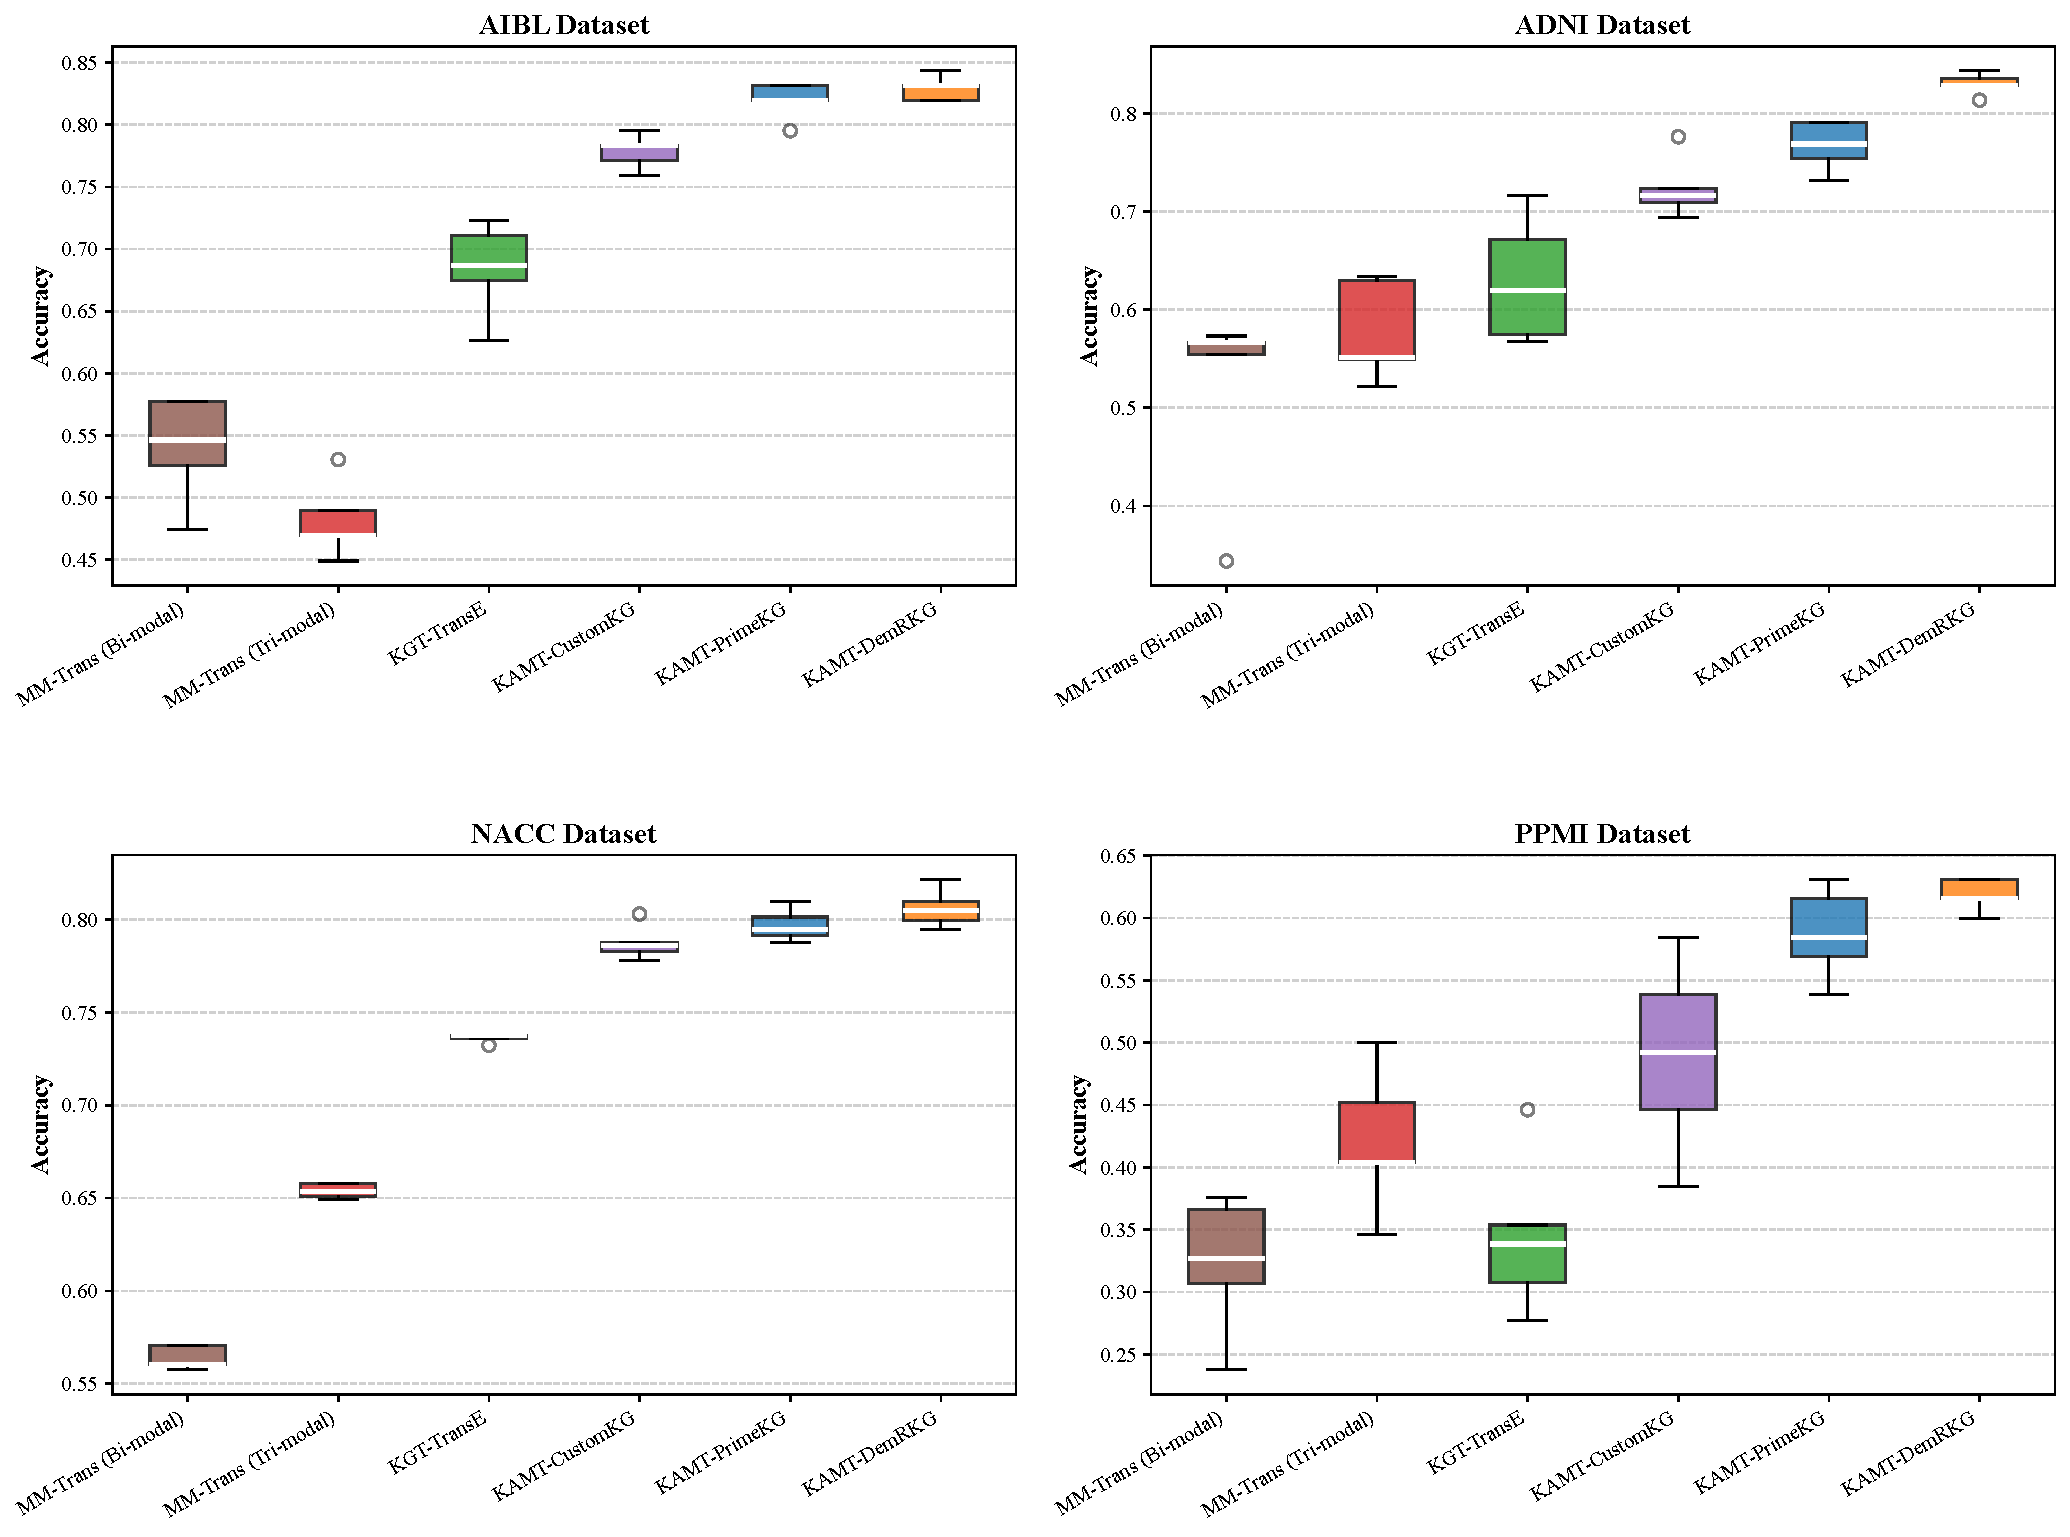
\includegraphics[width=0.9\linewidth]{Figures/箱型图-EN.pdf}
    \caption{Boxplot of prediction accuracy distribution across four independent cohorts.}
    \label{fig:accuracy_boxplot}
\end{figure}

\subsubsection{Semantic Preservation in Fine-Grained Alignment}

% TODO(method-audit): 核对本节标题及 point-to-point / fine-grained alignment 表述：当前每个模态编码为单个 Query token，知识读取是分支表征对多个实体的加权聚合。
% 后续 BM-EHR 与 MRI-临床融合各使用单个 Key/Value token，softmax 权重为 1；按分支信息融合描述，并区分维度匹配与字段级语义对齐。
    Fine-grained diagnosis can degrade when architectures impose aggressive compression (e.g., information bottlenecks), especially for dense text or detailed clinical scales (e.g., demographics in EHR and UPDRS in BioMarker). KAMT therefore enforces strict dimensional matching between Queries and Keys, enabling a point-to-point alignment between clinical observations and DemRKG nodes. Meanwhile, the knowledge injection is coupled with the energy-constrained refinement in \cref{eq:energy_min}, which helps keep the aligned representations consistent with observed clinical measurements while preserving fine-grained semantics.

\subsubsection{Clinical Limitations and Real-World Applicability}

Real-world deployment is still limited by reliance on complete cross-sectional snapshots, partial loss of topological detail in the current structural representation, and the lack of explicit causal reasoning paths. Future work will explore missing-modality-aware longitudinal modeling, higher-dimensional graph representations to preserve edge-level semantics, and path-tracking strategies to reconstruct interpretable reasoning chains.

%\section{Data availability}

    %\textcolor{blue}{The Parkinson’s Progression Markers Initiative (PPMI, http://www.ppmi-info.org/) database and the Parkinson’s Disease Biomarkers Program (PDBP, https://pdbp.ninds.nih.gov/) database used in this study are both accessible through AMP-PD (https://amp-pd.org/). To access clinical and omics data at the AMP-PD Tier 2 level, users are required to complete a data use agreement and submit an online application.}
	

%\section*{Code availability}

	%This M$^2$STGAT method is implemented in Python and available in Github (https://github.com/ZJ-BMDmining/M2DGAT).


    
%\section*{Acknowledgment}

	%This work is sponsored by National Natural Science Foundation of China(62302455, 62172369), Special Support Plan for High-level Talents in Zhejiang Province(2021R52019) and Natural Science Foundation of Zhejiang Province, China(LQ24F030007).
	
	

%\section*{References}
\bibliographystyle{IEEEtran}
\bibliography{references.bib}




\vfill

\end{document}


